\documentclass[a4paper, landscape, 6pt]{article}

% --------------------------------------------------------------------------------------------------------------------------------------------------------------------------
\input{./package_and_config.tex}

\def\subject{Mathematik}
\def\semester{2. Semester}
\def\author{Michael Graber, Joshua Kohler, Sven Gahlinger, Oliver Schütz}
\def\cols{3}

% Useful packages
\usepackage{amsmath}
\usepackage{graphicx}
\usepackage[colorlinks=true, allcolors=blue]{hyperref}
\usepackage{makecell}
\usepackage{adjustbox}
\usepackage{pgfplots}

\title{Mathe 2 Cheatsheet}

\cheatsheet{
    \section{Analysis}
    \subsection{Trigonometrie}
    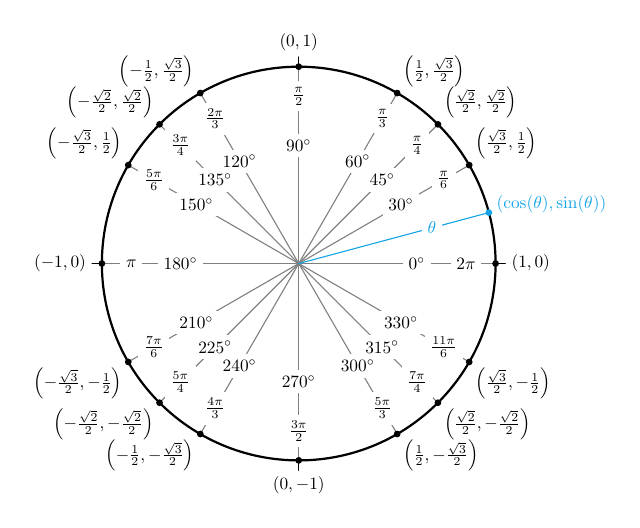
\begin{tikzpicture}[scale=2.5, transform shape, cap=round,>=latex, every node/.style={scale=0.25}] 
    % draw the coordinates
    \draw[-] (-1.05cm,0cm) -- (1.05cm,0cm);
    \draw[-] (0cm,-1.05cm) -- (0cm,1.05cm);

    % draw the unit circle
    \draw[thick] (0cm,0cm) circle(1cm);

    \foreach \x in {0,30,45,60,90,120,135,150,180,210,225,240,270,300,315,330} {
            % lines from center to point
            \draw[gray] (0cm,0cm) -- (\x:1cm);
            % dots at each point
            \filldraw[black] (\x:1cm) circle(0.4pt);
            % draw each angle in degrees
            \draw (\x:0.6cm) node[fill=white] {$\x^\circ$};
    }

    \draw[Cerulean](0cm,0cm) -- (15:1cm);
    \filldraw[Cerulean] (15:1cm) circle(0.4pt);
    \draw (15:0.7cm) node[Cerulean,fill=white] {$\theta$};
    \draw (13:1cm) node[above right,Cerulean] {$\left(\cos(\theta), \sin(\theta)\right)$};

    % draw each angle in radians
    \foreach \x/\xtext in {
        30/\frac{\pi}{6},
        45/\frac{\pi}{4},
        60/\frac{\pi}{3},
        90/\frac{\pi}{2},
        120/\frac{2\pi}{3},
        135/\frac{3\pi}{4},
        150/\frac{5\pi}{6},
        180/\pi,
        210/\frac{7\pi}{6},
        225/\frac{5\pi}{4},
        240/\frac{4\pi}{3},
        270/\frac{3\pi}{2},
        300/\frac{5\pi}{3},
        315/\frac{7\pi}{4},
        330/\frac{11\pi}{6},
        360/2\pi}
            \draw (\x:0.85cm) node[fill=white] {$\xtext$};

    \node[right] at (0:1.05cm) {$\left(1,0\right)$};
    \node[above] at (90:1.05cm) {$\left(0,1\right)$};
    \node[left] at (180:1.05cm) {$\left(-1,0\right)$};
    \node[below] at (270:1.05cm) {$\left(0,-1\right)$};

    \foreach \x/\xtext/\y in {
        150/-\frac{\sqrt{3}}{2}/\frac{1}{2},
        135/-\frac{\sqrt{2}}{2}/\frac{\sqrt{2}}{2},
        120/-\frac{1}{2}/\frac{\sqrt{3}}{2}}
            \draw (\x:1cm) node[above left] {$\left(\xtext,\y\right)$};

    
    \foreach \x/\xtext/\y in {
        30/\frac{\sqrt{3}}{2}/\frac{1}{2},
        45/\frac{\sqrt{2}}{2}/\frac{\sqrt{2}}{2},
        60/\frac{1}{2}/\frac{\sqrt{3}}{2}}
            \draw (\x:1cm) node[above right] {$\left(\xtext,\y\right)$}; 
    
    \foreach \x/\xtext/\y in { 
        210/-\frac{\sqrt{3}}{2}/-\frac{1}{2},
        225/-\frac{\sqrt{2}}{2}/-\frac{\sqrt{2}}{2},
        240/-\frac{1}{2}/-\frac{\sqrt{3}}{2} }
            \draw (\x:1cm) node[below left] {$\left(\xtext,\y\right)$};

    \foreach \x/\xtext/\y in {
        330/\frac{\sqrt{3}}{2}/-\frac{1}{2},
        315/\frac{\sqrt{2}}{2}/-\frac{\sqrt{2}}{2},
        300/\frac{1}{2}/-\frac{\sqrt{3}}{2}}
            \draw (\x:1cm) node[below right] {$\left(\xtext,\y\right)$};
\end{tikzpicture}
    \input{../Snippeds/Tigonometrie/unitcircle_2.tex}
    \begin{tabularx}{\linewidth}{|X|X|X|X|}
    \hline
    \textbf{Sin} & \textbf{Cos} & \textbf{Tan} & \textbf{Cot}\\
    \hline
    \textbf{G} & \textbf{A} & \textbf{G} & \textbf{A}\\
    \hline
    \textbf{H} & \textbf{H} & \textbf{A} & \textbf{G}\\
    \hline
\end{tabularx}

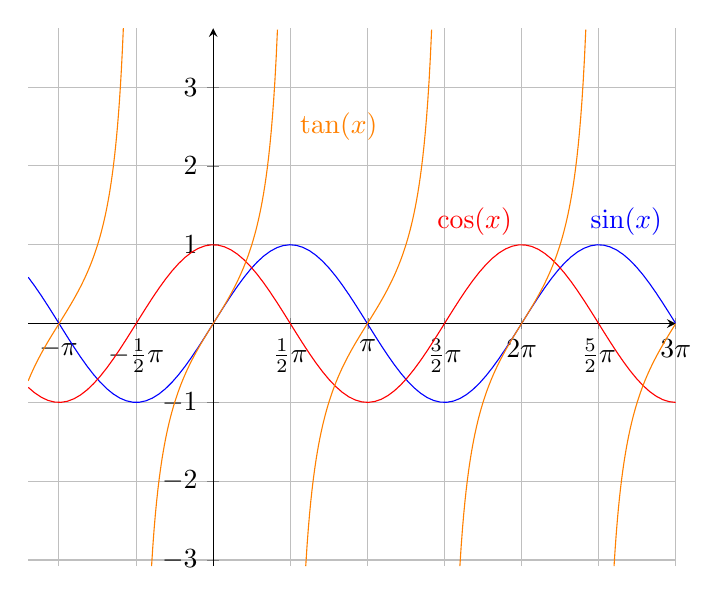
\begin{tikzpicture}
\begin{axis}[enlargelimits=false,
             axis lines=middle,
             scale=1.2,
             xtick={-3.15159, -1.57080, 0,
                     1.57080,  3.15159, 4.71239,
                     6.28318,  7.85398, 9.42478 }, 
             xticklabels={$-\pi$, $-\frac{1}{2}\pi$, 0,
                          $\frac{1}{2}\pi$, $\pi$, $\frac{3}{2}\pi$,
                          $2\pi$, $\frac{5}{2}\pi$, $3\pi$ },
             ytick={-3,-2,-1,0,1,2,3},
             grid=major, % only a grid on the defined ticks
             samples=100 % number of points
             ]
 
  % sin
  \addplot[blue,no marks,domain=-1.2*pi:3*pi]{sin(deg(x))}; % deg to convert radians
  \node[right=10pt,above] at (axis cs:5*pi/2,1){\color{blue}$\sin(x)$};
 
  % cos
  \addplot[red,no marks,domain=-1.2*pi:3*pi] {cos(deg(x))};
  \node[above left] at (axis cs:2*pi,1){\color{red}$\cos(x)$};
 
  % tan, multiple parts because of singularities
  \addplot[orange,no marks,domain=-1.2*pi:-0.583*pi, ]{tan(deg(x))};
  \addplot[orange,no marks,domain=-0.4*pi:5*pi/12,   ]{tan(deg(x))};
  \addplot[orange,no marks,domain=27*pi/45:17*pi/12, ]{tan(deg(x))};
  \addplot[orange,no marks,domain=1.6*pi:29*pi/12,   ]{tan(deg(x))};
  \addplot[orange,no marks,domain=2.6*pi:36*pi/12,   ]{tan(deg(x))};
  \node[right] at (axis cs:pi/2,2.5){\color{orange}$\tan(x)$};
 
\end{axis}
\end{tikzpicture}
    \subsection{Integrale}
    \subsubsection{Substitution}
\textbf{Normale Substitution}\\
\begin{flalign}
    \int_{a}^{b} f(g(x)) dx \quad | \quad u(x) = g(x) \quad &| \quad u'(x) = g'(x) \quad | \quad du = u'(x)\cdot dx \notag&\\
    \int_{u(a)}^{u(b)} u(x) \frac{1}{u'(x)} \,du \quad &| \quad dx = \frac{1}{u'(x)} \,du&\label{eq:Substitution}\\\notag
\end{flalign}
Wenn nach einer Substitution noch ein x in der Gleichung vorhanden ist, muss dieses in ein u umgewandelt werden.

\begin{flalign}
    \int \frac{e^{2x}}{1+e^{2}} \,dx \quad | \quad u = 1 + e^{x} \quad &| \quad u' = e^{x} \quad | \quad du = e^{x} \,dx \Leftrightarrow du = \frac{1}{e^{x}}&\notag\\
    \int \frac{e^{2x}}{u} \cdot \frac{1}{e^{x}} \,du = \int \frac{e^{x}}{u} \,du \quad &| \quad u = 1 + e^{x} \Leftrightarrow e^{x} = u - 1&\notag\\
    \int \frac{u - 1}{u} \,du = \int \frac{u}{u} - \frac{1}{u} \,du &= \int 1 - \frac{1}{u} \,du = \underline{\underline{u - \ln|u| + c}} &\notag
\end{flalign}\\

\textbf{Umgekehrte Substitution (Example)}\\

\begin{flalign}
    \int_{0}^{1} \sqrt{1 - x^2}\, dx \quad &| \quad x = \sin{u} \notag \quad | \quad x' = \cos{u} \notag&\\
    \int_{0}^{\frac{\pi}{2}} \sqrt{1 - \sin^2{u}} \cdot \cos{u}\,du \quad &| \quad dx = \cos{u}\, du \Leftrightarrow   du = \frac{1}{\cos{u}}\, dx \notag&\\
    \int_{0}^{\frac{\pi}{2}} \cos^2{u}\, du \quad =& \quad \left[\frac{u}{2} +  \frac{\sin{2u}}{4}\right]_{0}^{\pi/2} = \frac{\pi}{4} + 0 = \frac{\pi}{4}&\notag
\end{flalign}
    % https://en.wikipedia.org/wiki/List_of_integrals_of_trigonometric_functions#Integral_over_a_full_circle
\subsubsection{Standardintegrale}
\begin{multicols}{2}
    \begin{flalign}
        &\textbf{Standartintegrale}&\notag\\
        &\int m \,dx = m \cdot x + q&\\
        &\int a^{x} \,dx = \frac{a^{x}}{\ln{x}} + c&\\
        &\int{e^{x}} \,dx = e^x&\\ 
        &\int{x^{p}} \,dx = \frac{1}{p+1} \cdot x^{p+1} + c \quad n \ne -1&\\
        &\int{x^{-1}} \,dx = \int{\frac{1}{x}} \,dx = \ln|x| + c&\\
        &\int_{x_0}^{x_E}{x^{-1}} \,dx = \int{\frac{1}{x}} \,dx = \ln{\frac{x_E}{x_0}}&
    \end{flalign}
    \begin{flalign}
        &\textbf{Sinus}&\notag\\
        &\int{\sin{x} \cdot \cos{x}}\, dx = \frac{1}{2} \cdot \sin^2{x} + c&\\
        &\int{\sin^2{x}} \,dx = \frac{1}{2} (x - \sin{x} \cdot \cos{x}) + c&\\
        &\int{\sinh{x}} \,dx = \cosh{x} + c&\\
        &\textbf{Cosinus}&\notag\\
        &\int{\frac{1}{\cos^2{x}} \,dx} = \int{1 + \tan^2{x}}&\notag\\
        & = \tan{x} + c&\\
        &\int{\cosh{x}}\,dx = \sinh{x} + c&\\
        &\int{\cot{x}}\, dx = \frac{1}{\tan{x}} + c&\notag\\
        &= \ln|\sin{x}| + c = \frac{\cos{x}}{\sin{x}} + c&\\
        &\int{\coth{x}}\, dx = \frac{\cosh{x}}{\sinh{x}} + c&\\
        &\textbf{Tangents}&\notag\\
        &\int{\tan{x}}\, dx = \frac{1}{\cot{x}} + c&\notag\\
        & = -\ln|\cos{x}| + c = \frac{\sin{x}}{\cos{x}} + c&\\
        &\int{\tanh{x}}\, dx = \frac{\sinh{x}}{\cosh{x}} + c&\\
        &\int{\frac{1}{1 + x^2}} \,dx = \arctan{x}&
    \end{flalign}
\end{multicols}


    \subsubsection{Integralfläche berechnen (analytisch)}
Sobald sich Funktionen schneiden, muss das Integral aufgeteilt werden.
Wenn die Fläche über/unter der X-Achse berechnet werden soll, kann diese als Funktion $g(x) = 0$ angesehen werden.

\begin{flalign}
    A = \int_{a}^{b}{|f(x) - g(x)|} \,dx \label{eq:Calculate_area}
\end{flalign}

\textcolor{red}{Scale Plot and make a better example}
\begin{center}
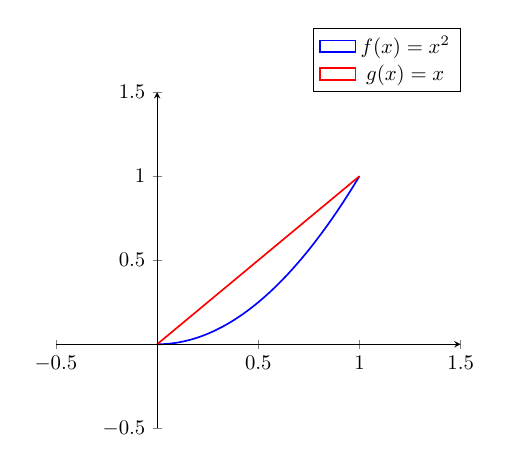
\begin{tikzpicture}[
    scale=0.75
    ]
    \begin{axis}[
        axis lines = middle,
        xmin = -0.5, xmax = 1.5,
        ymin = -0.5, ymax = 1.5,
        domain = 0:1,
        samples = 100,
        fill=blue!20,
        area style,
        legend style={at={(1,1)}, anchor=south east},
    ]
    \addplot[blue, thick] {x^2};
    \addplot[red, thick] {x};
    % \addplot[blue!20] fill between[of={x^2}, and={x}]; here is some compiling problem which I couldn't solve at the moment
    \legend{$f(x) = x^2$,$g(x) = x$}
    \end{axis}
\end{tikzpicture}
\end{center}

\textbf{Anleitung}
\begin{enumerate}
    \item Funktionen gleich setzen, um Nullstellen zu berechnen
    \item Integrale bilden
    \item Berechnen
\end{enumerate}
    \subsubsection{Volumenintegral berechnen}
\begin{flalign}
    &V = \pi \int_{a}^{b}{f(x)^{2}} \,dx \label{eq:Rotationsvolumen}&
\end{flalign}

\textbf{Anleitung}
\begin{enumerate}
    \item Rotation um Y-Achse \rightarrow \, Umkehrfunktion bestimmen
    \item Mit der Formel \ref{eq:Rotationsvolumen} das Volumen berechnen
\end{enumerate}
    \section{Komplexe Zahlen}
    \[
\arg(z) =
\begin{cases} 
    0                                                & \text{if } \Re(z) \geq 0 \land \Im(z) = 0 \quad | \quad \text{CASE 1}\\
    \arctan\left(\frac{\Im(z)}{\Re(z)}\right)        & \text{if } \Re(z) > 0 \land \Im(z) > 0 \quad | \quad \text{CASE 2}\\
    \frac{\pi}{2}                                    & \text{if } \Re(z) = 0 \land \Im(z) > 0 \quad | \quad \text{CASE 3}\\
    \arctan\left(\frac{\Im(z)}{\Re(z)}\right) + \pi  & \text{if } \Re(z) < 0 \qquad \qquad \qquad \quad| \quad \text{CASE 4}\\
    \pi                                              & \text{if } \Re(z) < 0 \land \Im(z) = 0 \quad | \quad \text{CASE 5}\\
    \frac{3\pi}{2}                                   & \text{if } \Re(z) = 0 \land \Im(z) < 0 \quad | \quad \text{CASE 6}\\
    \arctan\left(\frac{\Im(z)}{\Re(z)}\right) + 2\pi & \text{if } \Re(z) > 0 \land \Im(z) < 0 \quad | \quad \text{CASE 7}
\end{cases}
\]

\begin{center}
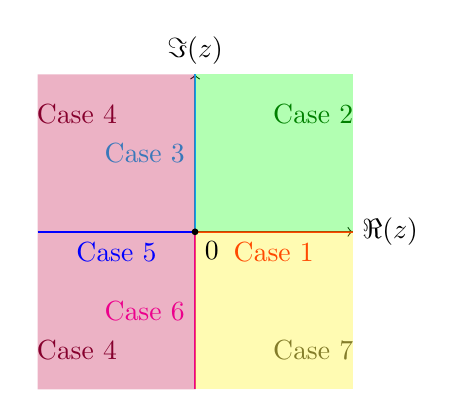
\begin{tikzpicture}[scale=1]
    % Axes
    \draw[->] (-2,0) -- (2,0) node[right] {$\Re(z)$};
    \draw[->] (0,-2) -- (0,2) node[above] {$\Im(z)$};
    
    % Regions
    % Case 1: Re(z) >= 0 and Im(z) = 0 (positive real axis)
    \draw[thick, red] (0,0) -- (2,0) node[midway, below] {Case 1};
    
    % Case 2: Re(z) > 0 and Im(z) > 0 (upper-right quadrant)
    \fill[green, opacity=0.3] (0,0) -- (0,2) -- (2,2) -- (2,0) -- cycle;
    \node[green!50!black] at (1.5,1.5) {Case 2};
    
    %  Case 3: Re(z) = 0 and Im(z) > 0 (positive imaginary axis)
    \draw[thick, cyan] (0,0) -- (0,2) node[midway, left] {Case 3};
    
    \fill[purple, opacity=0.3] (0,0) -- (0,2) -- (-2,2) -- (-2,-2) -- (0,-2) -- cycle;
    % Case 4: Re(z) < 0 and Im(z) > 0 (upper-left quadrant)
    \node[purple!70!black] at (-1.5,1.5) {Case 4};
    % Case 4: Re(z) < 0 and Im(z) < 0 (lower-left quadrant)
    \node[purple!70!black] at (-1.5,-1.5) {Case 4};
    
    % Case 5: Re(z) < 0 and Im(z) = 0 (negative real axis)
    \draw[thick, blue] (0,0) -- (-2,0) node[midway, below] {Case 5};
    
    % Case 6: Re(z) = 0 and Im(z) < 0 (negativ imaginary axis)
    \draw[thick, magenta] (0,0) -- (0,-2) node[midway, left] {Case 6};
    
    % Case 7: Re(z) > 0 and Im(z) < 0 (lower-right quadrant)
    \node[yellow!20!black] at (1.5,-1.5) {Case 7};
    \fill[yellow, opacity=0.3] (0,0) -- (0,-2) -- (2,-2) -- (2,0) -- cycle;
    
    % Origin
    \filldraw[black] (0,0) circle (1pt) node[below right] {$0$};
\end{tikzpicture}
\end{center}
\label{fig:Arg-cases}

    

\subsubsection{Koordinaten Arten}
\begin{flalign}
    &\textbf{Kartesische Koordinaten}& \notag \\
    &z = x + iy &\\[1ex]
    &\textbf{Polarkoordinaten} & \notag \\
    &\text{Umrechnung kartesisch} \to \text{polar:} & \notag \\
    &r = \sqrt{x^2 + y^2} & \notag \\
    &\varphi = \arctan\left(\frac{y}{x}\right) \quad (x \neq 0) & \notag \\[1ex]
    &\textbf{Komplexe Polarform} & \notag \\
    &\operatorname{cis} \varphi = \cos \varphi + i \sin \varphi & \notag \\
    &z = r \operatorname{cis} \varphi = r(\cos \varphi + i \sin \varphi) & \label{eq:polarform} \\[1ex]
    &\textbf{Euler-Form} & \notag \\
    &z = re^{i\varphi} \quad \text{(äquivalent zur Polarform)} & \label{eq:euler}
\end{flalign}

\begin{flalign}
    &x = r \cdot \cos{\phi} \quad|\quad y = r \cdot \sin{\phi}&\\
    &\varphi = \arctan{\frac{x}{y}}&\\
    &z = re^{i\varphi} = x + iy = r\cdot \operatorname{cis}{\varphi}&
\end{flalign}
    \subsubsection{Koordinaten Wechsel}

\begin{flalign}
    &\textbf{Kartesisch $\Rightarrow$ Polar}&\notag\\
    &
    &\textbf{Polar $\Rightarrow$ Kartesisch}&\notag\\
    &&\\
\end{flalign}
    \section{Lineare Algebra}
    \subsection{Vektoranalysis}
    \subsubsection{Kreuzprodukt}
\begin{minipage}{\linewidth}
    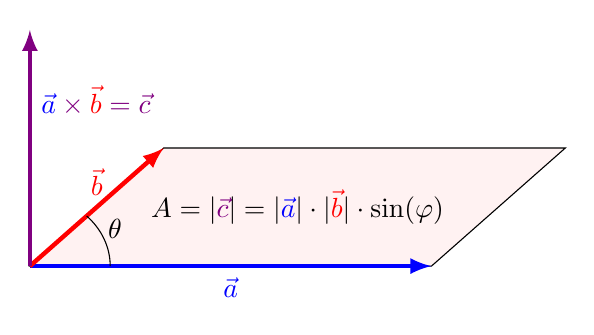
\begin{tikzpicture}[yscale=1.5, xscale=1.7, every node/.style={scale=1}]
    % Rechteck
    \draw[-,fill=white!95!red](0,0)--(3,0)--(4,1)--(1,1)--cycle;
    % Formel in der Fläche
    \node at (2,0.5) {$A = |\textcolor{violet}{\vec{c}} | = |\textcolor{blue}{\vec{a}}| \cdot |\textcolor{red}{\vec{b}}| \cdot \sin(\varphi)$};
    % a
    \draw[ultra thick,-latex,blue](0,0)--(3,0)node[midway,below]{$\vec{a}$};
    % b
    \draw[ultra thick,-latex,red](0,0)--(1,1)node[midway,above]{$\vec{b}$};
    % a x b
    \draw[ultra thick,-latex,blue!50!red](0,0)--(0,2)node[pos=0.7,right]{$\textcolor{blue}{\vec{a}} \times \textcolor{red}{\vec{b}} = \vec{c}$};
    \draw (0.6,0) arc [start angle=0,end angle=45,radius=0.6]
    node[pos=0.7,right]{$\theta$};
    \end{tikzpicture}
\end{minipage}
    \section{Variabletabbele}
    \section{Übungsaufgaben}
}


\end{document}